% =====================================================================
% ARTI5001 Assignment 3: Single-Speaker TTS on LJSpeech (report skeleton)
% Overleaf: New Project > Upload Project > zip of this report/ folder
%           (or Overleaf GitHub sync). Compiler: pdfLaTeX.
% LIMIT: 12 A4 pages INCLUDING references.
% Every \ph{...} is a placeholder. Every "HD:" comment is the rubric descriptor
% the section must satisfy. Delete the comments once a section is done.
% =====================================================================
\documentclass[11pt,a4paper]{article}
\usepackage[margin=2.2cm]{geometry}
\usepackage[T1]{fontenc}
\usepackage{lmodern,microtype}
\usepackage{graphicx,booktabs,tabularx,multirow,xcolor,enumitem}
\usepackage{amsmath}
\usepackage{tikz}
\usetikzlibrary{positioning,arrows.meta}
\usepackage[round]{natbib}          % Harvard (author-year) citations
\usepackage[hidelinks]{hyperref}
\setlist{nosep}

% Placeholder macro: renders as a red box so nothing unfinished slips through
\newcommand{\ph}[1]{\colorbox{red!12}{\textcolor{red!70!black}{\small\textsf{[#1]}}}}
% Owner tag shown next to headings while drafting; set to {} before submission
\newcommand{\owner}[1]{\hfill{\small\textcolor{gray}{(#1)}}}

\title{\textbf{Text-to-Speech on LJSpeech:\\ \ph{subtitle stating the controlled comparison}}}
\author{Group \ph{NN}\\[4pt]
\ph{Name 1} (\ph{a1xxxxxxx}) \quad \ph{Name 2} (\ph{a1xxxxxxx}) \quad \ph{Name 3} (\ph{a1xxxxxxx})\\[4pt]
ARTI5001 Generative Artificial Intelligence, Adelaide University}
\date{\ph{DD} November 2026}

\begin{document}
\maketitle
\thispagestyle{empty}

% ---------------------------------------------------------------------
\section*{Executive Summary}\owner{Member 1}
% HD (2.1): concise (<=1 page), NON-TECHNICAL. Must cover:
%  (1) the problem  (2) the delivered system  (3) practical value
%  (4) feasibility / scaling  (5) what the results MEAN (not just numbers)
\noindent\textbf{Problem.} \ph{why converting text to natural speech matters; who benefits}

\noindent\textbf{What we built.} \ph{plain-language description: type a sentence, get a voice recording}

\noindent\textbf{What we found.} \ph{headline result in everyday terms, e.g. ``option B is X\% easier to understand and still speaks faster than real time on a laptop''}

\noindent\textbf{Practical value.} \ph{accessibility, audiobooks, assistants; cost per hour of audio}

\noindent\textbf{Feasibility and scaling.} \ph{runs on \ldots; what full-scale deployment would need}

\noindent\textbf{Recommendation.} \ph{which variant to use and why, in one sentence}
\newpage

% ---------------------------------------------------------------------
\section{Introduction and Problem Framing}\owner{Member 1}
% HD (2.1): aim and scope framed CLEARLY.
\ph{context: TTS and its applications \citep{shen2018tacotron2}}

\noindent\textbf{Aim.} \ph{one sentence}

\noindent\textbf{Scope.} \ph{single speaker; subset size; compute budget; what is out of scope}

\noindent\textbf{Research question.} \ph{How does \emph{<controlled variable>} affect intelligibility, quality and speed?}

\noindent\textbf{Contributions.}
\begin{itemize}
  \item \ph{reproducible LJSpeech pipeline with a fixed split (seed 42, 90/5/5)}
  \item \ph{controlled comparison expA vs expB}
  \item \ph{multi-metric evaluation: RTF, latency, WER, MCD (+ listening test)}
\end{itemize}

% ---------------------------------------------------------------------
\section{Background and Related Work}\owner{All, from docs/RESEARCH.md}
% Short (~0.5 page). Positions our choice among the alternatives. Only cite papers you have read.
\ph{autoregressive (Tacotron 2) vs non-autoregressive (FastSpeech 2) vs end-to-end (VITS); neural vocoders (WaveNet, HiFi-GAN); evaluation (MOS, ASR-WER)}

% ---------------------------------------------------------------------
\section{System Design}\owner{Member 2}
% HD (2.2): CLEAR DIAGRAM + role of EACH module + justify choices by linking
%            CONSTRAINTS (compute/time/data) -> DECISIONS (front-end/acoustic/vocoder) -> GOALS.
\begin{figure}[h]
\centering
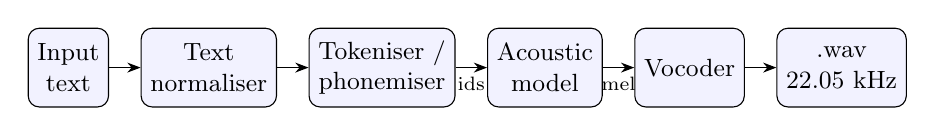
\begin{tikzpicture}[node distance=4mm, box/.style={draw, rounded corners, align=center, minimum height=10mm, font=\small, fill=blue!5}, >=Stealth]
  \node[box] (t) {Input\\text};
  \node[box, right=of t] (n) {Text\\normaliser};
  \node[box, right=of n] (p) {Tokeniser /\\phonemiser};
  \node[box, right=of p] (a) {Acoustic\\model};
  \node[box, right=of a] (v) {Vocoder};
  \node[box, right=of v] (w) {.wav\\22.05 kHz};
  \draw[->] (t) -- (n); \draw[->] (n) -- (p); \draw[->] (p) -- node[below,font=\scriptsize]{ids} (a);
  \draw[->] (a) -- node[below,font=\scriptsize]{mel} (v); \draw[->] (v) -- (w);
\end{tikzpicture}
\caption{End-to-end pipeline. \ph{replace module names with the actual components; mark which are pretrained vs trained by us}}
\label{fig:pipeline}
\end{figure}

\subsection{Modules}
\begin{tabularx}{\linewidth}{@{}lXl@{}}
\toprule
Module & Role & Input $\rightarrow$ Output \\ \midrule
Text front-end & \ph{normalisation, tokens} & string $\rightarrow$ \ph{ids, len $L$} \\
Acoustic model & \ph{...} & ids $\rightarrow$ mel $[80\times T]$ \\
Vocoder & \ph{...} & mel $\rightarrow$ waveform \\ \bottomrule
\end{tabularx}

\subsection{Design Justification}
\begin{tabularx}{\linewidth}{@{}lXX@{}}
\toprule
Constraint & Decision & Consequence / evidence \\ \midrule
Compute: \ph{device} & \ph{fine-tune pretrained / small model} & \ph{train time, \S\ref{sec:results}} \\
Time: 1 week & \ph{...} & \ph{...} \\
Data: \ph{n} utterances & \ph{...} & \ph{...} \\
Goal: real-time, intelligible & \ph{...} & \ph{RTF, WER} \\ \bottomrule
\end{tabularx}

\noindent\ph{alternatives considered and why rejected}

% ---------------------------------------------------------------------
\section{Experimental Design}\owner{Member 3 (+ Member 1 for data protocol)}
% HD (2.3): >=2 controlled experiments, motivated by a clear comparison goal;
%           protocol (split/seed/pre-processing) EXPLICIT and CONSISTENT WITH THE CODE.
\subsection{Data Protocol}\owner{Member 1}
\ph{LJSpeech 1.1 \citep{ito2017ljspeech}: 13{,}100 clips, 23.9 h, 22{,}050 Hz. Split 90/5/5 (11{,}790/655/655), seed 42, split hash \texttt{\ph{md5}}. Training subset of \ph{n} drawn from train only. Text: \ph{normalisation}. Audio: \ph{trim top\_db, sample-rate policy}.}

\subsection{Hypothesis and Controlled Variable}
\ph{``Changing X from A to B will improve/worsen Y because Z.'' Everything else held fixed.}

\subsection{Training and Selection Protocol}
\ph{steps/epochs, batch size, LR, optimiser, validation frequency, checkpoint selection rule, logging, hardware, wall-clock time}

\begin{table}[h]
\centering
\caption{Experiment settings (the controlled change is in bold).}
\label{tab:settings}
\begin{tabular}{@{}lll@{}}
\toprule
Setting & expA (baseline) & expB \\ \midrule
Model / vocoder & \ph{} & same \\
\textbf{Controlled variable} & \textbf{\ph{A}} & \textbf{\ph{B}} \\
Training utterances & \ph{} & \ph{} \\
Steps / batch / LR & \ph{} & same \\
Split / seed & 90/5/5, 42 & same \\
Training time & \ph{} & \ph{} \\ \bottomrule
\end{tabular}
\end{table}

% ---------------------------------------------------------------------
\section{Results and Evaluation}\label{sec:results}\owner{Member 3}
% HD (2.4): objective metric(s) reported CLEARLY *and INTERPRETED*; qualitative evidence
%           (audio) USED to support a reasoned TRADE-OFF discussion (quality vs speed, data vs quality).
\subsection{Objective Metrics}
\begin{table}[h]
\centering
\caption{Objective results on the test split (mean $\pm$ std over \ph{N} runs; device: \ph{device}). Arrows show the better direction.}
\label{tab:results}
\begin{tabular}{@{}lccccc@{}}
\toprule
Exp. & RTF $\downarrow$ & Latency (s) $\downarrow$ & WER (\%) $\downarrow$ & CER (\%) $\downarrow$ & MCD (dB) $\downarrow$ \\ \midrule
expA & \ph{} & \ph{} & \ph{} & \ph{} & \ph{} \\
expB & \ph{} & \ph{} & \ph{} & \ph{} & \ph{} \\
Ground truth & -- & -- & \ph{} & \ph{} & 0 \\ \bottomrule
\end{tabular}
\end{table}
\noindent\ph{interpretation: what each difference MEANS; is it larger than run-to-run variance?}

\subsection{Qualitative Evidence}\owner{Member 1}
\ph{listening observations tied to specific files, e.g. \texttt{expA\_04.wav} vs \texttt{expB\_04.wav}; blind A/B preference counts; spectrogram figure}
% \begin{figure}[h]\centering\includegraphics[width=\linewidth]{figures/spec_compare.png}\caption{...}\end{figure}

\subsection{Trade-offs}
\ph{quality vs speed; data size vs quality; training cost vs gain; include figures/tradeoff.png}

% ---------------------------------------------------------------------
\section{Error Analysis and Improvements}\owner{Member 2}
% HD (2.5): >=2 COMMON failure modes + realistic, TECHNICALLY GROUNDED improvements.
\begin{tabularx}{\linewidth}{@{}lXXX@{}}
\toprule
Failure mode & Evidence (wav / WER) & Cause & Proposed fix \\ \midrule
\ph{1} & \ph{} & \ph{} & \ph{} \\
\ph{2} & \ph{} & \ph{} & \ph{} \\
\ph{3 (optional)} & \ph{} & \ph{} & \ph{} \\ \bottomrule
\end{tabularx}

% ---------------------------------------------------------------------
\section{Conclusion and Recommendations}\owner{Member 1}
% HD (2.5): CLEAR recommendation of the preferred variant + deployment/scaling + future work.
\noindent\textbf{Recommendation.} \ph{preferred variant + evidence}

\noindent\textbf{Deployment and scaling.} \ph{full-dataset training estimate, CPU vs GPU serving, throughput, model size}

\noindent\textbf{Limitations and future work.} \ph{...}

% ---------------------------------------------------------------------
\bibliographystyle{agsm}   % Harvard style (available on Overleaf)
\bibliography{references}

\appendix
\section{Contribution Statement}
\begin{tabularx}{\linewidth}{@{}lXc@{}}
\toprule
Member & Contribution (code / report / slides) & Share \\ \midrule
\ph{Name 1} & 1.1 data pipeline, attribution; Exec summary, Intro, Conclusion; slides: data & 33\% \\
\ph{Name 2} & 1.2 TTS pipeline; System design, Error analysis; slides: architecture + demo & 33\% \\
\ph{Name 3} & 1.3 experiments, 1.4 metrics; Experiments, Results; slides: results & 33\% \\ \bottomrule
\end{tabularx}

\section{AI Use Statement}
\ph{tools used, what for (e.g. brainstorming, debugging, language polishing), example prompts; all final content verified by the group}

\end{document}
